% A0 portrait poster, using the SFB 1294 template's portrait design.
% Content and figures adapted from ../poster_cristina/poster_retreat_2026.tex.
% Scientific claims and the required funding acknowledgement need final review.
\documentclass[english,UP]{sfb1294_1-poster}

\usepackage[oldboxesoff]{poster-boxes}
\usepackage{amsmath,amssymb,mathtools}
\usepackage{booktabs}
\usepackage{array}
\usepackage{graphicx}
\usepackage{xcolor}

\newcommand{\sigmoid}{\sigma}
\newcommand{\posterfigure}[3]{%
  \begin{minipage}[t]{0.48\linewidth}\centering
    \textbf{#1}\par\vspace{0.5mm}
    \includegraphics[width=\linewidth,height=#3,keepaspectratio]{#2}
  \end{minipage}%
}

\begin{document}
\titlebox{}%
{Bayesian Inference for Spatial Poisson Models\protect\\[0.5mm]
 \normalsize Exact posterior sampling by data augmentation and application to earthquake catalogues}%
{Toni Luhdo, Cristina Ch\'avez Chong, Matthias Holschneider}
\pagecolor{light-gray}

\begin{pspicture}(0,0)(\contentswidth,\contentsheight)

% ------------------------------------------------------------------
% LEFT COLUMN: MODEL, SAMPLER, EARTHQUAKE DATA, CONCLUSIONS
% ------------------------------------------------------------------
\rput[tl](3mm,255mm){%
  \postertabbox{white}{\fbsdefault}{0.48\contentswidth}{\large Spatial Poisson model}{%
    \footnotesize\raggedright
    We model events in spatial cell $i$ by
    \[n_i\mid f_i\sim\operatorname{Poisson}(\lambda_i),\qquad
      \lambda_i=\lambda\sigmoid(f_i),\quad
      \sigmoid(f)=\frac{1}{1+e^{-f}}.\]
    The latent field has a Gaussian prior,
    $f\sim\mathcal N(\mu,Q^{-1})$, where $Q$ introduces spatial dependence.
    The scale parameter $\lambda$ has a Gamma prior.
    The posterior $p(f\mid n)\propto p(n\mid f)p(f)$ is non-Gaussian because
    of the Poisson--sigmoid likelihood.
  }%
}

\rput[tl](3mm,210mm){%
  \postertabbox{white}{\fbsdefault}{0.48\contentswidth}{\large Data augmentation}{%
    \footnotesize\raggedright
    Two auxiliary variables turn the latent-field update into a Gaussian draw:
    \[f^{(t)}\ \longrightarrow\ k\ \longrightarrow\ \omega\
      \longrightarrow\ f^{(t+1)}.\]
    First sample auxiliary counts and then P\'olya--Gamma variables:
    \[k_i\sim\operatorname{Poisson}\!\left(\lambda\sigmoid(-f_i)\right),
      \qquad \omega_i\sim\operatorname{PG}(n_i+k_i,f_i).\]
  }%
}

\rput[tl](3mm,171mm){%
  \postertabbox{white}{\fbsdefault}{0.48\contentswidth}{\large Gaussian update and computation}{%
    \footnotesize\raggedright
    After augmentation,
    \[f\mid n,k,\omega\sim
      \mathcal N(m_{\mathrm{post}},Q_{\mathrm{post}}^{-1}),\]
    \[Q_{\mathrm{post}}=Q+\Omega,\quad
      \Omega=\operatorname{diag}(\omega_1,\ldots,\omega_N),\]
    \[m_{\mathrm{post}}=Q_{\mathrm{post}}^{-1}(Q\mu+\kappa),\quad
      \kappa_i=\frac{n_i-k_i}{2}.\]
    The spatial prior precision $Q$ is sparse. Adding diagonal $\Omega$
    preserves sparsity, allowing sparse Cholesky factorisation instead of
    a dense covariance matrix.
  }%
}

\rput[tl](3mm,124mm){%
  \postertabbox{white}{\fbsdefault}{0.48\contentswidth}{\large Uniform ergodicity}{%
    \footnotesize\raggedright
    Let $K(f'\mid f)$ be the transition kernel. For $\alpha>0$, $\delta>0$
    and $Q\succ0$, there are $\varepsilon>0$ and a density $h$ on
    $\mathbb R^M$ such that
    \[K(f'\mid f)\geq\varepsilon h(f'),\qquad f,f'\in\mathbb R^M.\]
    Consequently, the marginal latent-field chain is uniformly ergodic.
  }%
}

\rput[tl](3mm,90mm){%
  \postertabbox{white}{\fbsdefault}{0.48\contentswidth}{\large Italian earthquake catalogue}{%
    \footnotesize\raggedright
    \begin{minipage}[t]{0.37\linewidth}\vspace{0pt}\centering
      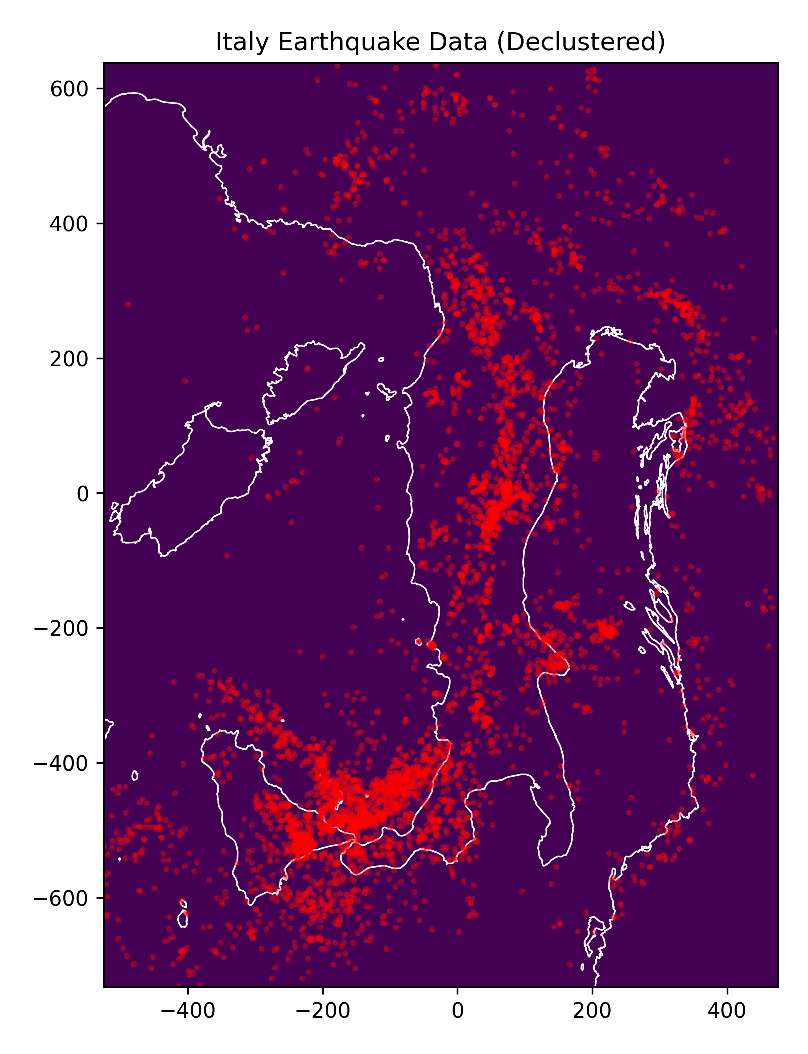
\includegraphics[width=\linewidth,height=30mm,keepaspectratio]
        {figures/italy_italy_earthquake_data_bin_5km_declustered.eps}
    \end{minipage}\hfill
    \begin{minipage}[t]{0.61\linewidth}\vspace{0pt}\centering
      \scriptsize
      \begin{tabular}{@{}lrr@{}}\toprule
        Statistic & Original & NND \\
        & catalogue & declustered \\\midrule
        Events & 11,327 & 4,943 \\
        Occupied cells & 3,518 & 3,230 \\
        Cells $\geq10$ & 135 & 16 \\
        Cells $\geq15$ & 89 & 5 \\
        Maximum count & 279 & 23 \\
        Variance / mean & 49.26 & 2.66 \\\bottomrule
      \end{tabular}
    \end{minipage}
    \par\vspace{1mm}
    NND declustering reduces highly populated cells while preserving much
    of the catalogue's spatial footprint.
  }%
}

\rput[tl](3mm,32mm){%
  \postertabbox{white}{\fbsdefault}{0.48\contentswidth}{\large Conclusions}{%
    \footnotesize\raggedright
    Exact data augmentation gives tractable Gaussian updates. Synthetic
    experiments recover the main spatial structures. The Italy posterior
    shows coherent seismicity patterns. Sampling provides uncertainty
    beyond MAP estimation.\par
    \textit{Preliminary results / work in progress.}
  }%
}

% ------------------------------------------------------------------
% RIGHT COLUMN: TWO SYNTHETIC EXPERIMENTS, POSTERIOR, REFERENCES
% ------------------------------------------------------------------
\rput[tl](107.7mm,255mm){%
  \postertabbox{white}{\fbsdefault}{0.48\contentswidth}{\large Experiment 1: elongated bars}{%
    \footnotesize\raggedright
    \posterfigure{True rate}{figures/synthetic_bars_true_rate_rho_3_lam_12_var_4.eps}{24mm}
    \hfill
    \posterfigure{Observed counts}{figures/synthetic_bars_observed_counts_rho_3_lam_12_var_4.eps}{24mm}
    \par\vspace{1mm}
    \posterfigure{Posterior mean}{figures/synthetic_bars_posterior_mean_rate_rho_3_lam_12_var_4.eps}{24mm}
    \hfill
    \posterfigure{Mean $-$ MAP}{figures/synthetic_bars_posterior_mean_minus_map_rho_3_lam_12_var_4.eps}{24mm}
    \par\vspace{1mm}
    The sampler identifies elongated high-rate structures despite strong
    Poisson noise. Differences are largest near sharp, narrow structures,
    where the spatial prior smooths the field.
  }%
}

\rput[tl](107.7mm,171mm){%
  \postertabbox{white}{\fbsdefault}{0.48\contentswidth}{\large Experiment 2: compact block}{%
    \footnotesize\raggedright
    \posterfigure{True rate}{figures/synthetic_block_true_rate_rho_2_lam_12_var_4.eps}{24mm}
    \hfill
    \posterfigure{Observed counts}{figures/synthetic_block_observed_counts_rho_2_lam_12_var_4.eps}{24mm}
    \par\vspace{1mm}
    \posterfigure{Posterior mean}{figures/synthetic_block_posterior_mean_rate_rho_2_lam_12_var_4.eps}{24mm}
    \hfill
    \posterfigure{Mean $-$ MAP}{figures/synthetic_block_posterior_mean_minus_map_rho_2_lam_12_var_4.eps}{24mm}
    \par\vspace{1mm}
    The compact high-rate region is recovered; the spatial prior smooths
    its sharp boundary.
  }%
}

\rput[tl](107.7mm,92mm){%
  \postertabbox{white}{\fbsdefault}{0.48\contentswidth}{\large Posterior inference in Italy}{%
    \footnotesize\raggedright
    \posterfigure{Posterior mean $f$}{figures/italy_posterior_mean_f_bin_5km_declustered.eps}{21mm}
    \hfill
    \posterfigure{Posterior sd $f$}{figures/italy_posterior_sd_f_bin_5km_declustered.eps}{21mm}
    \par\vspace{1mm}
    \begin{minipage}[t]{0.35\linewidth}\vspace{0pt}\centering
      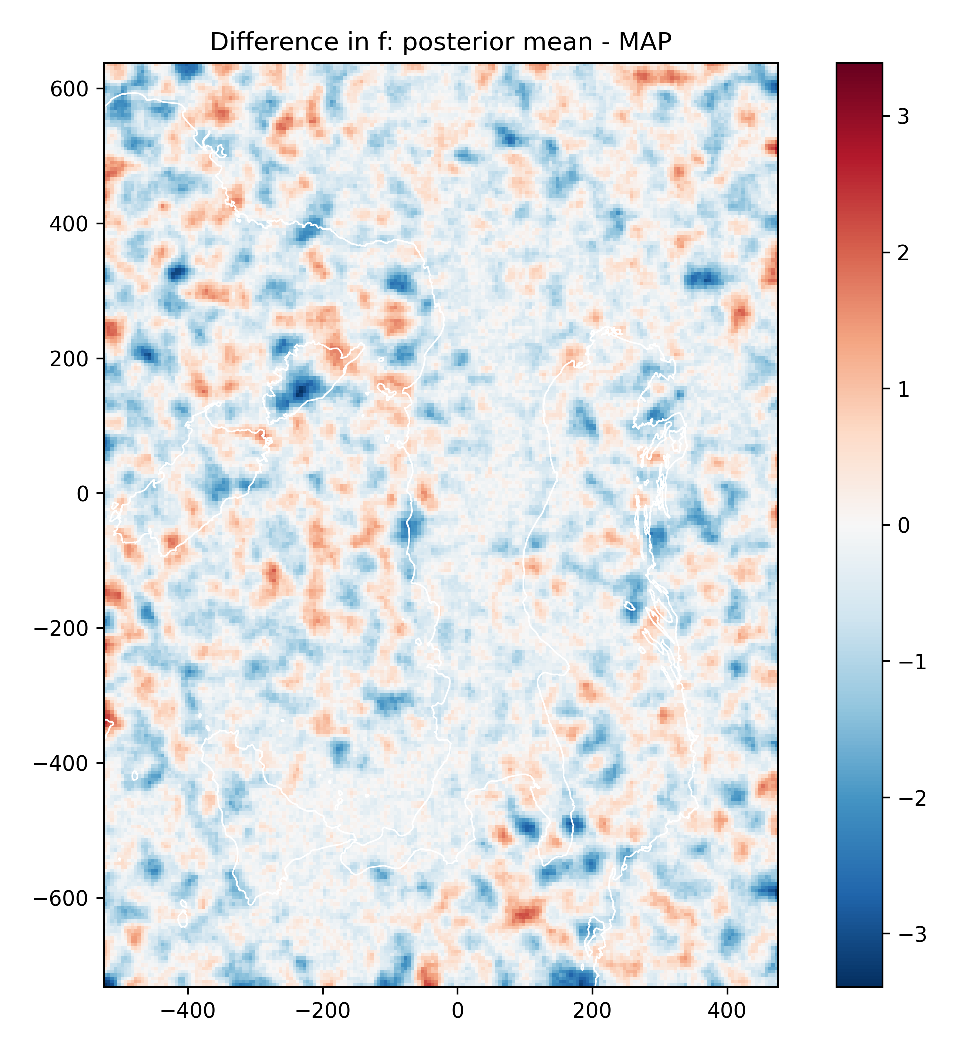
\includegraphics[width=\linewidth,height=18mm,keepaspectratio]
        {figures/italy_difference_f_bin_5km_declustered.eps}
    \end{minipage}\hfill
    \begin{minipage}[t]{0.62\linewidth}\vspace{0pt}
      \textbf{MAP versus full posterior.} MAP and posterior mean show
      similar broad-scale structures. Sampling additionally describes
      spatial uncertainty and reveals posterior asymmetry.
    \end{minipage}
  }%
}

\rput[tl](107.7mm,32mm){%
  \postertabbox{white}{\fbsdefault}{0.48\contentswidth}{\large References}{%
    \scriptsize\raggedright
    Choi \& Hobert (2013), \textit{The P\'olya--Gamma Gibbs sampler for
    Bayesian logistic regression is uniformly ergodic}, EJS.\par
    Polson, Scott \& Windle (2013), \textit{Bayesian inference for logistic
    models using P\'olya--Gamma latent variables}.\par
    Zaliapin \& Ben-Zion, nearest-neighbor methods for earthquake
    clustering and declustering.
  }%
}

\end{pspicture}
\end{document}
